\subsection{Beam-to-rigid body contact for yarn-mandrel contact-friction interactions}
\subsubsection{Test case description}
Following the numerical test on mortar line contact for yarn-to-mandrel interactions, the dynamic simulation shall now be studied. A beam-to-rigid body contact formulation with friction based on a collocation approach has been implemented to study the dynamics of yarn deposition on a mandrel surface. The neutral axis of the beam is represented by proxy discrete spherical collision geometries \cite{tasora2020geometrically} (of radius $r_s$ = radius of the beam). The mandrel surface is treated as the master plane and the collision elements as the slave. For the robust handling of a large number of frictional impacts, Newton-type solvers may suffer from ill-conditioning and singularity issues in the Jacobian. Therefore, a Gau{\ss}-Seidel solver is exploited which is well-suited for such problems.\\

The time discrete equations are solved using the decoupled version of the nonsmooth generalized-$\alpha$ time integration scheme \cite{cosimo2020robust} with the Gau{\ss}-Seidel solver So-bogus \cite{daviet2011hybrid}. Three decoupled sub-problems are solved using the splitting strategy as $\Delta \vectorbold{q}_{n+1} = \Delta \vectorbold{\Tilde{q}}_{n+1} + \vectorbold{U}_{n+1}$ and $\vectorbold{v}_{n+1} = \vectorbold{\Tilde{v}}_{n+1} + \vectorbold{W}_{n+1}$, where, $\Delta \vectorbold{\Tilde{q}}_{n+1}$ and $\vectorbold{\Tilde{v}}_{n+1}$ are smooth displacements and velocities, and $\vectorbold{U}_{n+1}$ and $\vectorbold{W}_{n+1}$ are position corrections and velocity jumps. 

\subsubsection{Simulation setup}
The transient simulation of the contact-friction interactions between a slender beam winding around a cylindrical rigid body is performed using the Odin multibody dynamics research code \cite{odin2022}. The beam of radius $r_y = 0.001$ m and with length $l_y = 4$ m and material properties $(E = 90$ GPa, $\nu = 0.27$ and $\rho = 2670$ kg/m$^3$) has been used for winding around a cylindrical rigid body of radius  $r_m = 0.4$ m and length $l_m = 4$ m. The beam is discretized using 50 finite elements and spherical collision elements are attached to the nodes of the beam. A stiffness-proportional Rayleigh damping has been used for structural damping. \\
 

\subsubsection{Results}
The investigation of the yarn-mandrel interactions has been performed in Figure \ref{fig:fricvalues} for one frictionless and two frictional cases ($\mu = 0.1$ and $0.4$). The time evolution of the position of the centre node of the beam (node 25) has been selected for the study. As expected in winding using a higher value of the friction coefficient ($\mu = 0.4)$, the sliding motion of the node is significantly postponed as compared to $\mu = 0.1$ and $0.0$. The simulation is performed for a total time $T = 8$ s with a time step size of $h = 0.005$ s.

\begin{figure}[h]
\centering
  \centering
  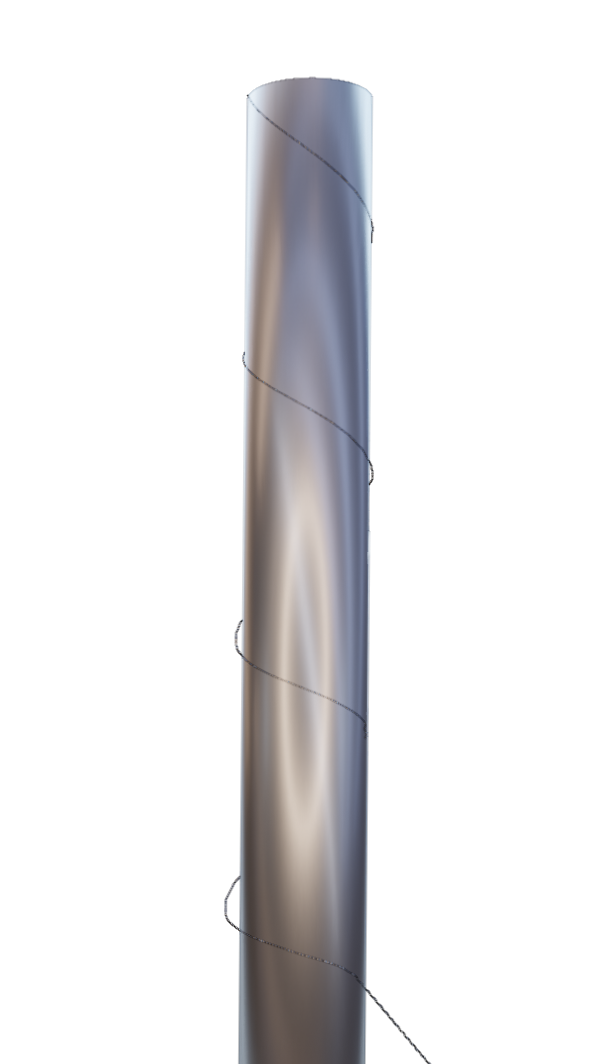
\includegraphics[width=0.27\linewidth]{figures/steel_mandrel_1.png}\\
  \centering
  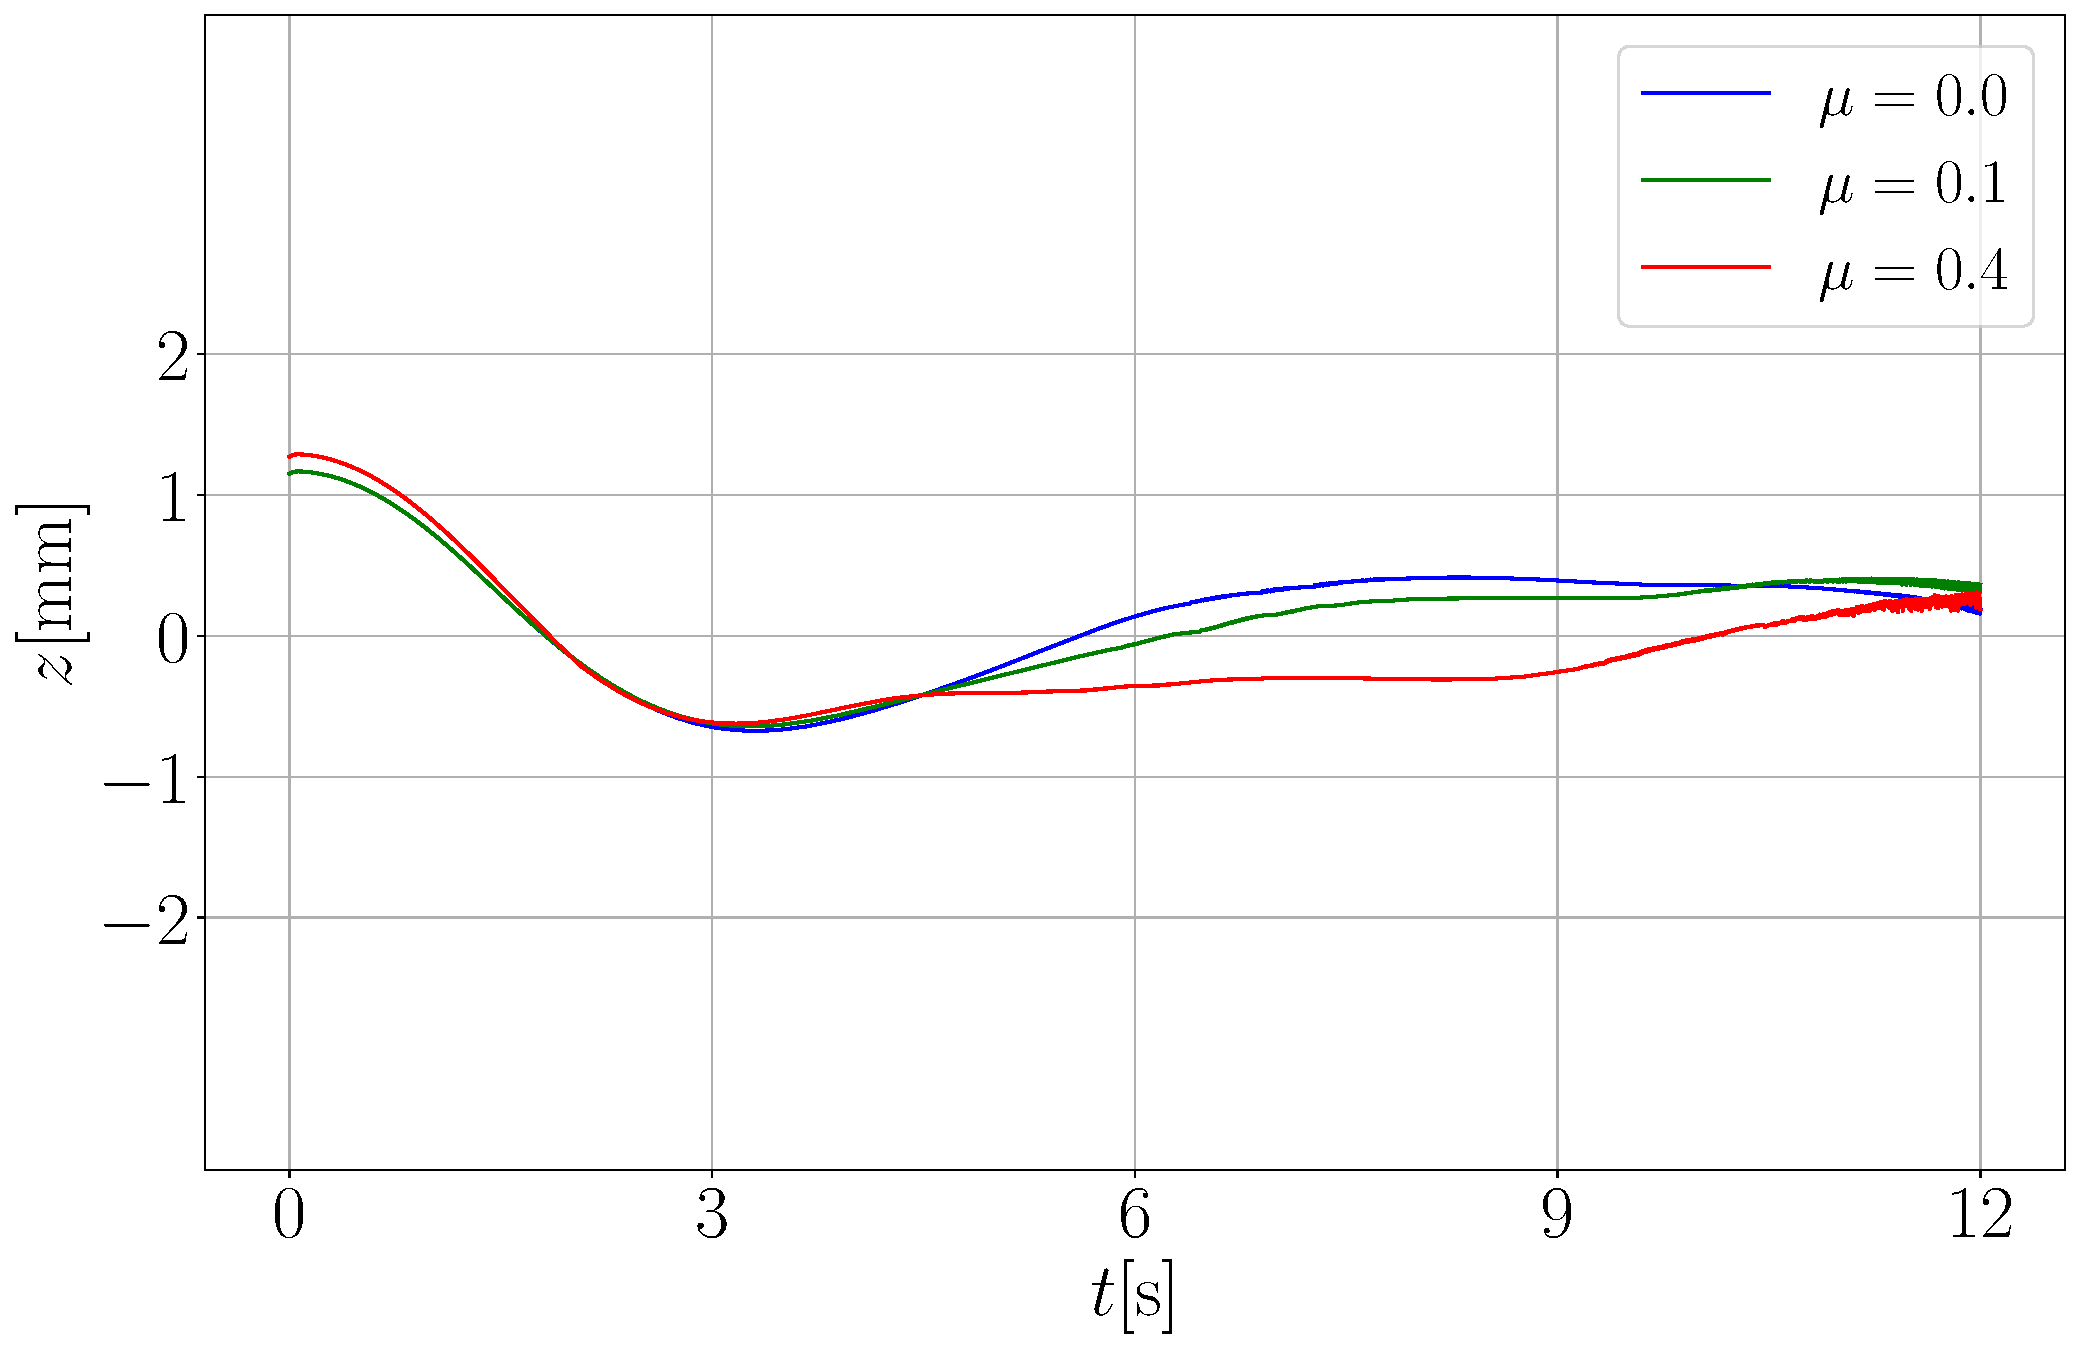
\includegraphics[width=0.47\linewidth]{figures/mu_compare.pdf}
\caption{Frictional dynamic yarn-to-mandrel interactions using beam-to-rigid body contact with a collocation approach. Time evolution of position of the centre node of the yarn along the longitudinal axis (z) of the mandrel for different friction coefficients.}
\label{fig:fricvalues}
\end{figure}



















